\documentclass[
    ../../Software_Engineering_Summary.tex,
]
{subfiles}

\externaldocument[ext:]{../../Software_Engineering_Summary.tex}
% Set Graphics Path, so pictures load correctly
\graphicspath{{../../}}

\begin{document}
\begin{samepage}
\subsection{Test Automation \& Tool Support}
\subsubsection{Automated Test Case Generation (ATCG)}
As writing test cases with good coverage is very time consuming, automated test case generation (ATCG) is often used instead.

\begin{defbox}
    [Fundamental Approaches]
    \begin{tabular}{r l}
        \defc{White Box}: & \parbox[t]{0.7\textwidth}{(\defc{Code Based}) Code of IUT is analyzed to achieve coverage. 
        \begin{itemize}
            \item \defc{Syntactic Approach:} Scan for conditions, evaluation. Achieves logic-based criteria.
            \item \defc{Symbolic Execution:} Unwinding CFG with symbolic values. Achieves structural coverage criteria.
            \subitem $\rightarrow$ \defc{Under-Approximation:} Unreached code.
        \end{itemize}} \\
        \defc{Black Box}: & Analysis of input data or model of IUT.
    \end{tabular}
\end{defbox}
\end{samepage}
\begin{samepage}
\subsubsection{Further Test Automation}
\begin{defbox}
    [Test Coverage Recording]
    \begin{enumerate}
        \item Instrument IUT
        \item Run test suite, collect information during test runs
        \item Analyze and display achieved coverage statistics
    \end{enumerate}
    \defc{Does not help with writing tests, but helps with knowing when to stop.}
\end{defbox}
\end{samepage}
\begin{defbox}
    [Test Oracle Synthesis]
    \begin{itemize}
        \item \defc{Human Oracle:} Time consuming and error-prone
        \item \defc{Verdict as Code (assert):} Need expertise, hard to maintain
    \end{itemize}
    $\rightarrow$ Write test oracle in \defc{formal specification language}, sythesize code from specification
\end{defbox}
\begin{samepage}    
\subsubsection{Automatic Static Verification Techniques}
\begin{defbox}
    [Static Checking]
    Typically based on CFG of IUT and constraint solving
    \begin{itemize}
        \item Runtime exceptions, liveness, information flow
        \item Fully automated
        \item Over-approximation, possibly many false positives
        \item Scales reasonably
    \end{itemize}
\end{defbox}
\end{samepage}
\begin{defbox}
    [Bug Finding]
    Based on pattern matching and heuristics
    \begin{itemize}
        \item Fast, scales well, handles full Java
        \item Over- and Under approximation (false positives and incomplete)
    \end{itemize}

    \defc{SpotBugs} is a static analysis tool utilizing bug patterns to find bugs in Java programs. It works at a byte code level.

    It sources its bug patterns from \textbf{complex language features}, \textbf{misunderstood API methods or invariants} and \textbf{typos and wrong usage of operators}
\end{defbox}

\begin{samepage}
\subsubsection{Formal Verification}

\begin{defbox}
    [Formal Approaches]
    \begin{itemize}
        \item Mathematical Foundation (logic and set theory)
        \item Sound relative to formal model (strong guarantee)
        \item Not necessarily complete (not all true properties can be proven)
    \end{itemize}
\end{defbox}

Often checked for by external programs that use either \defc{Model Checking} or \defc{Deductive Verification} by feeding it the source code and the formal specifications.
\end{samepage}

\begin{samepage}
\subsubsection{Design-by-Contract}
\begin{codebox}
    [Design-by-Contract Example in JML]
    \begin{lstlisting}[firstnumber=1,language=Java]
/*@ private normal_behavior
    // What needs to be true for this method to work correctly
    requires 0 <= low <= up <= a.length;
    requires (\forall int x,y;
            0 <= x < y < a.length; a[x] <= a[y]);
    // What this method guarantees to be true after execution
    ensures \result == -1 || low <= \result < up;
    ensures (\exists int idx;
            low <= idx < up; a[idx] == v) ?
        \result >= low && a[\result] == v
        : \result == -1;
    // What the method may modify
    assignable \nothing;
    // Specifies the termination metric
    measured_by up - low;
@*/
private int binSearch(int v, int low, int up) {...}
\end{lstlisting}
\end{codebox}
\end{samepage}
\begin{defbox}
    [Design-by-Contract]
    Formal specification:
    \begin{itemize}
        \item Pre- and Postconditions, side effects for each method
        \item Class and loop invariants
    \end{itemize}

    Verification tool proves that each method
    \begin{itemize}
        \item fulfills its contract in all possible runs
        \item preserves loop and object invariants
    \end{itemize}
\end{defbox}

\begin{samepage}
\subsubsection{Java Modelling Language (JML)}
JML is a \defc{contract-based specification language} tailored to java

\begin{defbox}
    [General JML Philosophy]
    Integrate
    \begin{itemize}
        \item JML specification
        \item Java implementation
    \end{itemize}
    within a single language
\end{defbox}

JML is not external to Java, but integrated
\end{samepage}
\begin{samepage}
\subsubsection{Deductive Verification}
\begin{defbox}
    [Working Principle: Path Exploration]
    \defc{Symbolic execution} explores all paths in CFG of straight-line programs (no jumps, no loops, no method calls)
    \begin{itemize}
        \item Finite number of paths
        \item Uses symbolic values to represent all inputs
        \item Loops approximated by all invariants
    \end{itemize}
\end{defbox}
\end{samepage}
\begin{defbox}
    [Scalability of Deductive Verification]
    Approximate effect of a method call with a contract
    \begin{itemize}
        \item During symbolic execution, replace called method with contract
        \item Substitution and first-order deduction instead of path exploration
    \end{itemize}
\end{defbox}

\begin{defbox}
    [Symbolic Execution Example]
    \centering
    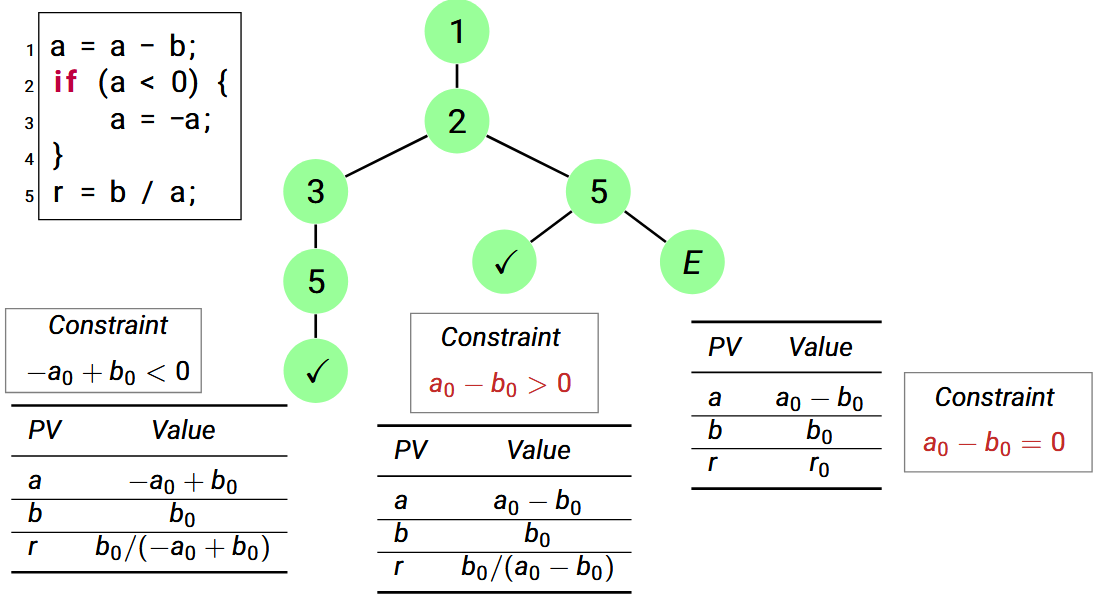
\includegraphics[width=0.8\textwidth]{Pics/11/SymbolicExecution.png}
\end{defbox}
\end{document}